\documentclass{article}
%%%%%%%%%%%%%%%%%%%%%%%%%%%%%%%%%%%%%%%%%%%%%%%%%%%%%%%%%%%%%%%%%%%%%%%%%%%%%%%%%%%%%%%%%%%%%%%%%%%%%%%%%
\usepackage{csquotes,xpatch}% recommended
\usepackage[backend=bibtex,
style=authoryear-comp,
sortcites=false,
maxbibnames=5,maxcitenames=2,
firstinits=true,
natbib=true,
]{biblatex}

\addbibresource{refs.bib}

% natbib = true: add comma between author and year
% firstinits: for first name initials in bibliography
\renewcommand{\postnotedelim}{ } % remove comma in post citation in autocite
%\addbibresource{refs.bib}
%%%%%%%%%%%%%%%%%%%%%%%%%%%%%%%%%%%%%%%%%%%%%%%%%%%%%%%%%%%%%%%%%%%%%%%%%%%%%%%%%%%%%%%%%%%%%%%%%%%%%%%%%

% Combine label and labelyear links
\xpatchbibmacro{cite}
{\usebibmacro{cite:label}%
	\setunit{\addspace}%
	\usebibmacro{cite:labelyear+extrayear}}
{\printtext[bibhyperref]{%
		\DeclareFieldAlias{bibhyperref}{default}%
		\usebibmacro{cite:label}%
		\setunit{\addspace}%
		\usebibmacro{cite:labelyear+extrayear}}}{}{}

% Include labelname in labelyear link
\xpatchbibmacro{cite}
{\printnames{labelname}%
	\setunit{\nameyeardelim}%
	\usebibmacro{cite:labelyear+extrayear}}
{\printtext[bibhyperref]{%
		\DeclareFieldAlias{bibhyperref}{default}%
		\printnames{labelname}%
		\setunit{\nameyeardelim}%
		\usebibmacro{cite:labelyear+extrayear}}}{}{}

% Access hyperref's citation link start/end commands
\makeatletter
\protected\def\blx@imc@biblinkstart{%
	\@ifnextchar[%]
	{\blx@biblinkstart}
	{\blx@biblinkstart[\abx@field@entrykey]}}
\def\blx@biblinkstart[#1]{%
	\blx@sfsave\hyper@natlinkstart{\the\c@refsection @#1}\blx@sfrest}
\protected\def\blx@imc@biblinkend{%
	\blx@sfsave\hyper@natlinkend\blx@sfrest}
\blx@regimcs{\biblinkstart \biblinkend}
\makeatother

\newbool{cbx:link}

% Include parentheses around labelyear in \textcite only in
% single citations without pre- and postnotes
\def\iflinkparens{%
	\ifboolexpr{ test {\ifnumequal{\value{multicitetotal}}{0}} and
		test {\ifnumequal{\value{citetotal}}{1}} and
		test {\iffieldundef{prenote}} and
		test {\iffieldundef{postnote}} }}

\xpatchbibmacro{textcite}
{\printnames{labelname}}
{\iflinkparens
	{\DeclareFieldAlias{bibhyperref}{default}%
		\global\booltrue{cbx:link}\biblinkstart%
		\printnames{labelname}}
	{\printtext[bibhyperref]{\printnames{labelname}}}}{}{}

\xpatchbibmacro{textcite}
{\usebibmacro{cite:label}}
{\iflinkparens
	{\DeclareFieldAlias{bibhyperref}{default}%
		\global\booltrue{cbx:link}\biblinkstart%
		\usebibmacro{cite:label}}
	{\usebibmacro{cite:label}}}{}{}

\xpretobibmacro{textcite:postnote}
{\ifbool{cbx:link}% patch 2.7+
	{\ifbool{cbx:parens}
		{\bibcloseparen\global\boolfalse{cbx:parens}}
		{}%
		\biblinkend\global\boolfalse{cbx:link}}
	{}}
{}
{\xpatchbibmacro{textcite}% patch earlier releases
	{\setunit{%
			\ifbool{cbx:parens}
			{\bibcloseparen\global\boolfalse{cbx:parens}}
			{}%
			\multicitedelim}}
	{\ifbool{cbx:link}
		{\ifbool{cbx:parens}
			{\bibcloseparen\global\boolfalse{cbx:parens}}
			{}%
			\biblinkend\global\boolfalse{cbx:link}}
		{}%
		\setunit{%
			\ifbool{cbx:parens}
			{\bibcloseparen\global\boolfalse{cbx:parens}}
			{}%
			\multicitedelim}}
	{}{}}
%%%%%%%%%%%%%%%%%%%%%%%%%%%%%%%%%%%%%%%%%%%%%%%%%%%%%%%%%%%%%%%%%%%%%%%%%%%%%%%%%%%%%%%%%%%%%%%%%%%%%%%%%
\DeclareNameAlias{sortname}{last-first} % last name first
\renewbibmacro{in:}{} % remove in: before journal

%%%%%%%%%%%%%%%%%%%%%%%%%%%%%%%%%%%%%%%%%%%%%%%%%%%%%%%%%%%%%%%%%%%%%%%%%%%%%%%%%%%%%%%%%%%%%%%%%%%%%%%%%
\usepackage{graphicx}
\usepackage{epstopdf} 
%%%%%%%%%%%%%%%%%%%%%%%%%%%%%%%%%%%%%%%%%%%%%%%%%%%%%%%%%%%%%%%%%%%%%%%%%%%%%%%%%%%%%%%%%%%%%%%%%%%%%%%%%
\usepackage{calrsfs}
\usepackage{physics}
\usepackage{mathtools}  
\usepackage{amsmath}
\usepackage{amssymb}
\usepackage{tabulary}
\usepackage{booktabs}
\usepackage{hyperref}
%%%%%%%%%%%%%%%%%%%%%%%%%%%%%%%%%%%%%%%%%%%%%%%%%%%%%%%%%%%%%%%%%%%%%%%%%%%%%%%%%%%%%%%%%%%%%%%%%%%%%%%%%
%\usepackage{chngcntr}
%\numberwithin{equation}{chapter}
%\counterwithin{figure}{chapter}
%%%%%%%%%%%%%%%%%%%%%%%%%%%%%%%%%%%%%%%%%%%%%%%%%%%%%%%%%%%%%%%%%%%%%%%%%%%%%%%%%%%%%%%%%%%%%%%%%%%%%%%%%
\setlength{\parindent}{2em}
\setlength{\parskip}{1em}

\linespread{1.6}
\usepackage{geometry}
\geometry{
	a4paper,
	total={134mm,225mm},
	left=38mm,
	top=35mm,
	headsep=.5in
}
\raggedbottom
%%%%%%%%%%%%%%%%%%%%%%%%%%%%%%%%%%%%%%%%%%%%%%%%%%%%%%%%%%%%%%%%%%%%%%%%%%%%%%%%%%%%%%%%%%%%%%%%%%%%%%%%%
\usepackage{blindtext}
\usepackage{ragged2e}
\usepackage{float}

\usepackage{epstopdf}
\usepackage{empheq} 

\usepackage{array}
\hypersetup{
	colorlinks
}
%%%%%%%%%%%%%%%%%%%%%%%%%%%%%%%%%%%%%%%%%%%%%%%%%%%%%%%%%%%%%%%%%%%%%%%%%%%%%%%%%%%%%%%%%%%%%%%%%%%%%%%%%
\usepackage{graphics}
\graphicspath{ {figures/} }
\renewcommand{\listfigurename}{List of figures}

\usepackage[labelfont=bf,justification=justified,singlelinecheck=false]{caption}
\captionsetup[figure]{name=Fig. ,labelsep=period}
\captionsetup[table]{labelsep=period}
\captionsetup[figure]{labelfont={bf},labelformat={default},labelsep=period,name={Fig.}}
%%%%%%%%%%%%%%%%%%%%%%%%%%%%%%%%%%%%%%%%%%%%%%%%%%%%%%%%%%%%%%%%%%%%%%%%%%%%%%%%%%%%%%%%%%%%%%%%%%%%%%%%%
\usepackage{array}
\usepackage{longtable}
\usepackage{xcolor}

\usepackage{comment}

\usepackage{enumitem}

\usepackage{wrapfig}
%%%%%%%%%%%%%%%%%%%%%%%%%%%%%%%%%%%%%%%%%%%%%%%%%%%%%%%%%%%%%%%%%%%%%%%%%%%%%%%%%%%%%%%%%%%%%%%%%%%%%%%%%
\usepackage{titlesec}

\titlespacing*{\section}
{0pt}{1ex plus .5ex minus .2ex}{.5ex plus .2ex}
\titlespacing*{\subsection}
{0pt}{0.5ex plus .5ex minus .2ex}{.5ex plus .2ex}
%\titlespacing*{\subparagraph}
%{0pt}{2.5ex plus 1ex minus .2ex}{1.3ex plus .2ex}

\setcounter{secnumdepth}{4}
\setcounter{tocdepth}{4}

\newcommand{\hsp}{\hspace{5pt}}

\titleformat{\section}[block]{\bfseries\large}{\thesection}{1em}{}
\titleformat{\subsection}[block]{\bfseries\itshape}{\thesubsection}{1em}{}


%\titleformat{\subsubsection}
%{\normalfont\normalsize\itshape}{\thesubsubsection}{1em}{}
%\titleformat{\subparagraph}[runin]
%{\itshape\normalsize}{\thesubparagraph}{1em}{}

%%%%%%%%%%%%%%%%%%%%%%%%%%%%%%%%%%%%%%%%%%%%%%%%%%%%%%%%%%%%%%%%%%%%%%%%%%%%%%%%%%%%%%%%%%%%%%%%%%%%%%%%%
\usepackage{subcaption}
\usepackage{bbm}
\usepackage{tabularx}
%%%%%%%%%%%%%%%%%%%%%%%%%%%%%%%%%%%%%%%%%%%%%%%%%%%%%%%%%%%%%%%%%%%%%%%%%%%%%%%%%%%%%%%%%%%%%%%%%%%%%%%%%
\definecolor{mycolor}{RGB}{207,42,40}
\AtBeginDocument{\hypersetup{citecolor=violet, linkcolor = mycolor}}

\usepackage{indentfirst}


%%%%%%%%%%%%%%%%%%%%%%%%%%%%%%%%%%%%%%%%%%%%%%%%%%%%%%%%%%%%%%%%%%%%%%%%%%%%%%%%%%%%%%%%%%%%%%%%%%%%%%%%

\DeclareMathAlphabet{\pazocal}{OMS}{zplm}{m}{n}
\newcommand{\bw}{\boldsymbol{w}}
\newcommand{\bp}{\boldsymbol{p}}
\newcommand{\bth}{\boldsymbol{\theta}}
\newcommand{\bA}{\boldsymbol{A}}
\newcommand{\cH}{\pazocal{H}}
\newcommand{\cN}{\pazocal{N}}
\newcommand{\cP}{\pazocal{P}}
\newcommand{\cD}{\pazocal{D}}
\newcommand{\cO}{\pazocal{O}}
\newcommand{\cL}{\pazocal{L}}


\setcounter{tocdepth}{3}
\begin{document}
	
	\sloppy
	
%%%%%%%%%%%%%%%%%%%%%%%%%%%%%%%%%%%%%%%%%%%%%%%%%%%%%%%%%%%%%%%%%%%%%%%%%%%%%%%%%%%%%%%%%%%%%%%%%%%%%%%%%
	\begin{center}	
		\large
		\textbf{Review of \textcite{fort2020deep}}\\
		\large
		Apostolos Psaros\\	
%		\today
%		July 10, 2020
	\end{center}
	\vskip 0.25in
	
%%%%%%%%%%%%%%%%%%%%%%%%%%%%%%%%%%%%%%%%%%%%%%%%%%%%%%%%%%%%%%%%%%%%%%%%%%%%%%%%%%%%%%%%%%%%%%%%%%%%%%%%%
%{\footnotesize
%\setlength{\parskip}{0.1em}
%\linespread{0.1}
%\tableofcontents
%\newpage}


%\setlength{\parskip}{1em}
%\linespread{1.6}
\section{Summary}\label{sec:introduction}
In this paper the authors show empirically what has been conjectured before:
Repeated optimization of a NN with different initialization leads to different weight vectors with similar training loss. 
Also, the NN evaluated at these different optima gives very different predictions. 
This is called diversity/disagreement of predictions.

On the other hand, recent techniques that use a single SGD to sample more weights for performing approximate Bayesian inference lead to very similar (not diverse) predictions. 
In this paper they study 4 such techniques which I will be calling ``4 sampling techniques'' for convenience. 

We knew that the 4 sampling techniques give similar predictions, but here is more empirical evidence. 
Note, however, that the 4 sampling techniques come at a very small or no additional cost as compared to a single optimization. 
Note also that if we use a cyclical learning schedule we may be able to visit other modes as well: see empirical evidence in Section 4.5 in \textcite{fort2019large}. 
However, \textcite{fort2020deep} have not tried to use cyclical learning schedule. 

Note: These results are for classification but I believe similar results we can get for regression. I have not looked into it yet. See Figure 11 in \textcite{wilson2020bayesian} for a starting point in function diversity for regression.

\section{Two definitions}
We will use cosine similarity in weight space (w-space) given as
\begin{equation}
	cos(\theta_1,\theta_2) = \frac{\theta_1^T\theta_2}{\norm{\theta_1}\norm{\theta_2}}
\end{equation}
and disagreement of 2 models in function space (f-space) given as
\begin{equation}
\frac{1}{N}\sum_{n=1}^{N}\boldsymbol{1}[f(x_n;\theta_1)\neq f(x_n;\theta_2)]
\end{equation}

\section{Discussion of figures}
\begin{figure}[H]
	\centering
	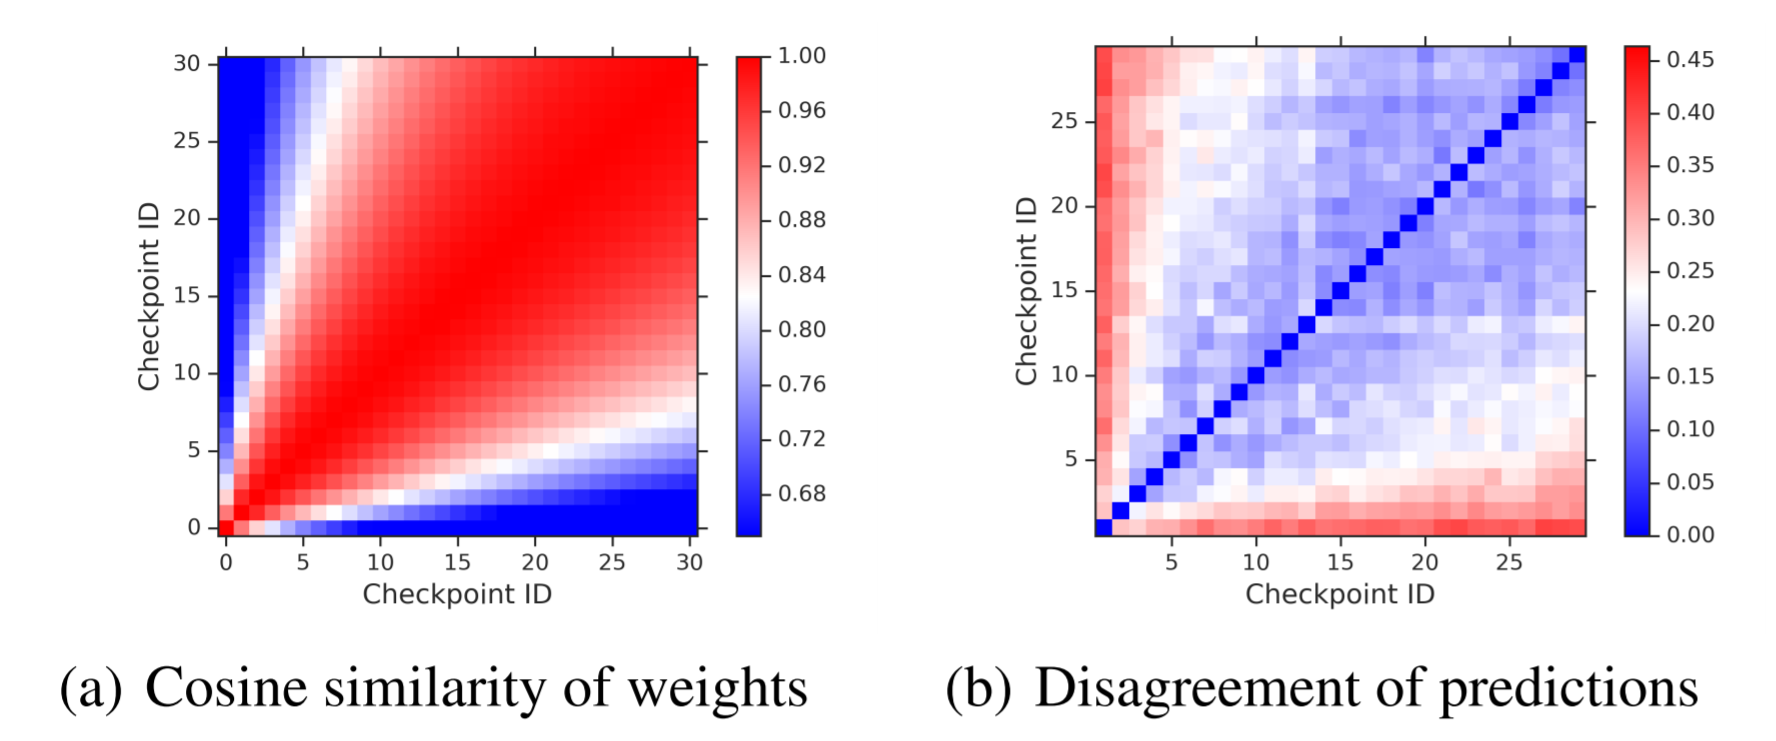
\includegraphics[width=0.7\linewidth]{./Figures/Figure2ab.png}
	\caption{Figure 2 a and b from the paper: 
		a) Cosine similarity of weights along an optimization trajectory. After checkpoint 10, weights within a trajectory are very similar.
	b) Disagreement of functions obtained along an optimization trajectory. After checkpoint 10, models predict very similar labels. Predictions are not very diverse.}
	\label{}
\end{figure}
\begin{figure}[H]
	\centering
	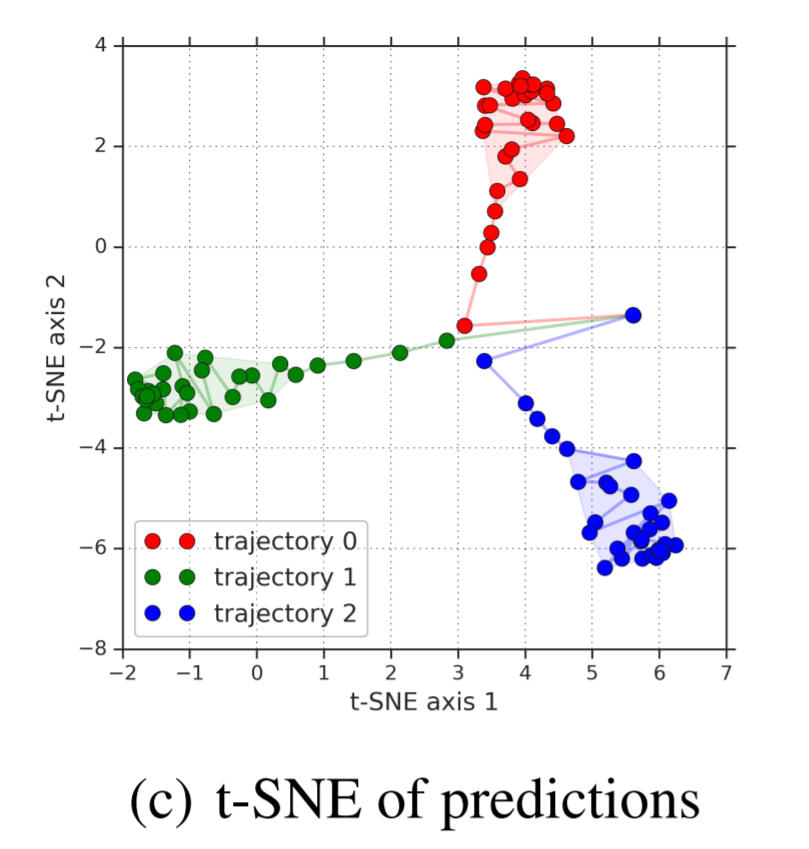
\includegraphics[width=0.5\linewidth]{./Figures/Figure2c.png}
	\caption{Figure 2 c from the paper: 
		2-D t-SNE projections of predictions obtained from weights along 3 different optimization trajectories. Projections corresponding to the same trajectory (color) are very close to each other but far from predictions from different trajectories. This shows that weights within a trajectory give rise to very similar predictive models but different trajectories give rise to very different models.}
	\label{}
\end{figure}
\begin{figure}
	\centering
	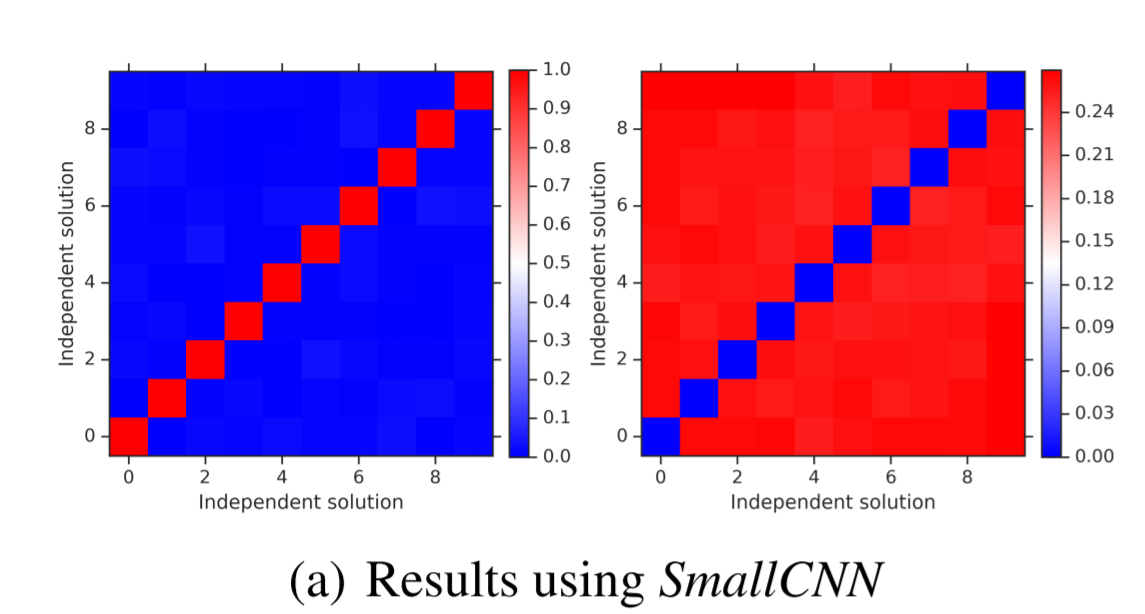
\includegraphics[width=0.7\linewidth]{./Figures/Figure3a.png}
	\caption{Figure 3 a from the paper: 
		Left: Cosine similarity between optima (final weights in each trajectory) from different optimization trajectory. Different optima are almost orthogonal to each other. Right: Corresponding predictive models/functions obtained disagree on predictions.}
	\label{}
\end{figure}
\begin{figure}
	\centering
	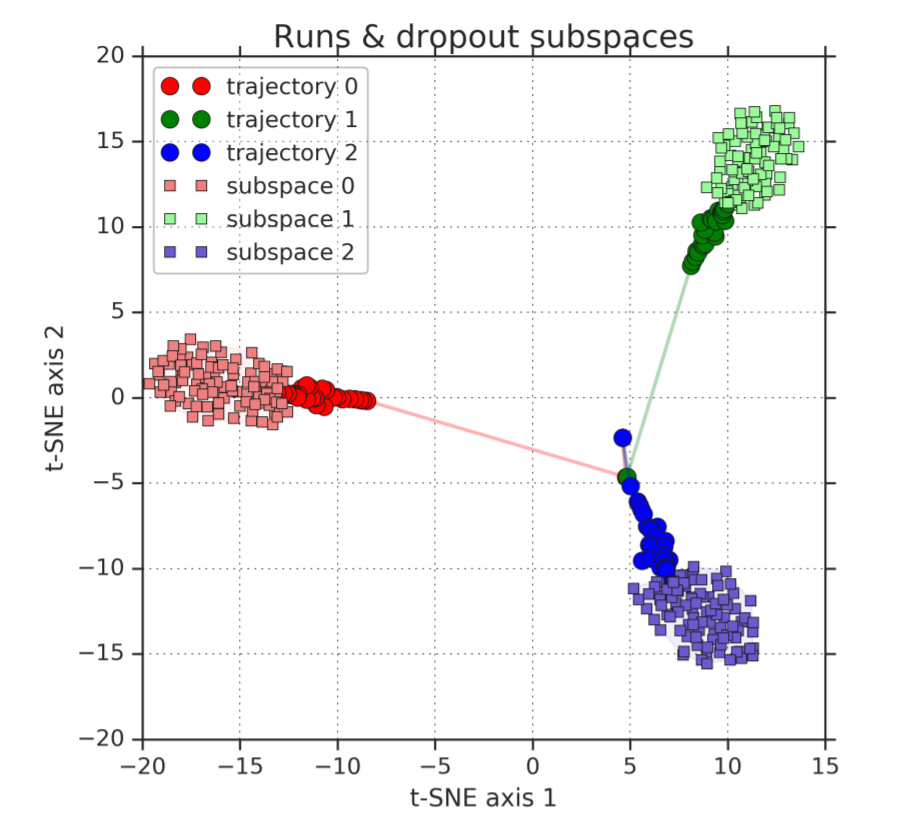
\includegraphics[width=0.7\linewidth]{./Figures/Figure4.png}
	\caption{Figure 4 from the paper: 
		2-D t-SNE projections of predictions obtained from 3 different optimization trajectories. Additional predictions (less opacity in figure) are added by using one of the 4 sampling techniques (here dropout). Remember these 4 sampling techniques at zero or low cost sample more weights along a single optimization trajectory. It is seen that the sampling techniques only help better explore a single mode and the predictions are not very diverse.}
	\label{}
\end{figure}
\begin{figure}
	\centering
	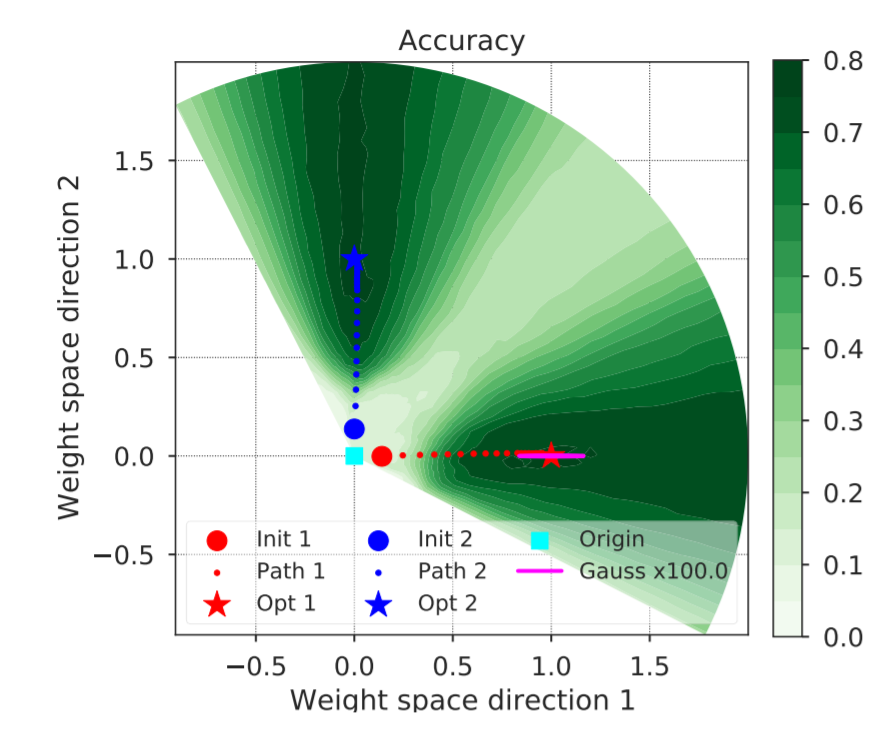
\includegraphics[width=0.7\linewidth]{./Figures/Figure5left.png}
	\caption{Figure 5 left from the paper: 
		Having 3 points in the w-space we can create a unique 2-D plane passing through these 3 points. See for example \textcite{li2018visualizing} and \textit{losslandscape.com} where they create a plane connecting one weight plus 2 random directions from it. In this figure the 3 points for creating a plane are the origin and the 2 optima (stars) found by 2 different optimization trajectories. The dots show the 2 trajectories as projected on this plane (as far as I understand it). It seems that because of high dimensionality the points along the optimization trajectories fall very close to the lines connecting the origin and the optima. It is also seen that the 2 optima achieve similar training loss while if we tried to connect the 2 optima with a straight line we would have to pass through a region of high loss. Connecting ``tunnels'' between 2 optima can be found with the techniques of \textcite{garipov2018loss} and \textcite{draxler2018essentially}. See also \textcite{fort2019large} for tunnels connecting M modes. These tunnels are useful because we can use the different weights in the tunnel for ensembling. In order to produce this plot we need to go at each pixel in the plot (corresponding to a weight vector) and compute its training loss. Finally, with pink you can see the different weights obtained by using one of the 4 sampling techniques. They are very close to the optimum of the 1st trajectory and they are orthogonal to the optimum of the 2nd trajectory.
	}
	\label{}
\end{figure}
\begin{figure}
	\centering
	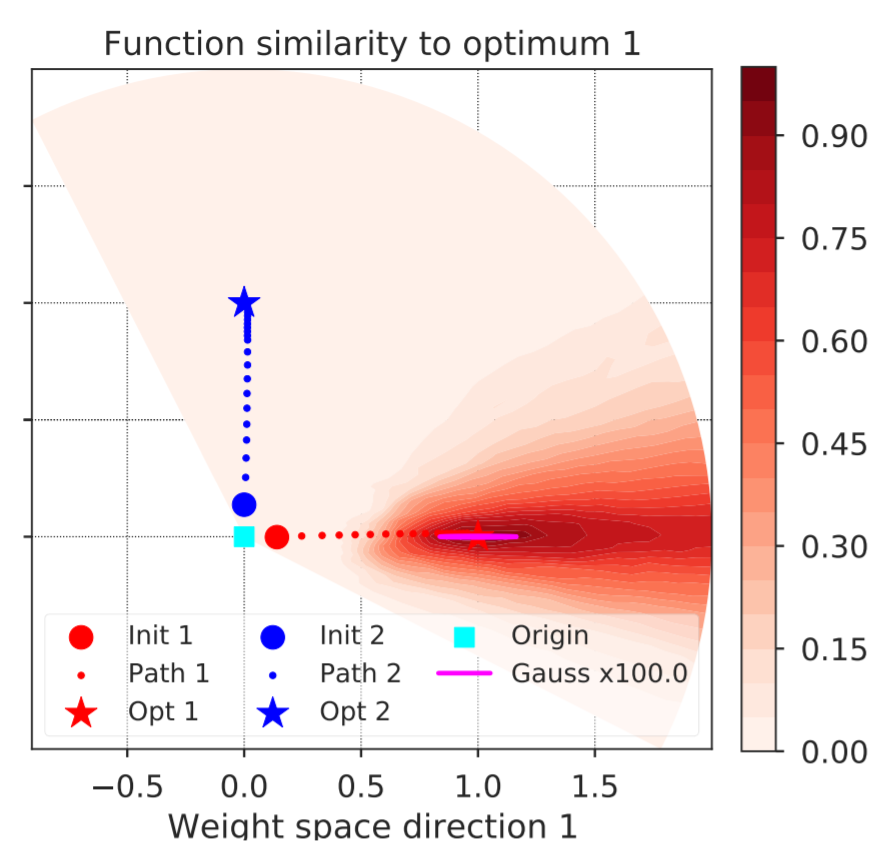
\includegraphics[width=0.7\linewidth]{./Figures/Figure5middle.png}
	\caption{Figure 5 middle from the paper: 
		Function similarity of each model in the plane as compared to the 1st optimum. This shows that when we leave the low loss valley around the weight the predictions are very different. Finally, with pink you can see the function similarities of the weights obtained by using one of the 4 sampling techniques. The functions obtained are very similar to the function obtained using the optimum of the 1st trajectory.}
	\label{}
\end{figure}
\begin{figure}
	\centering
	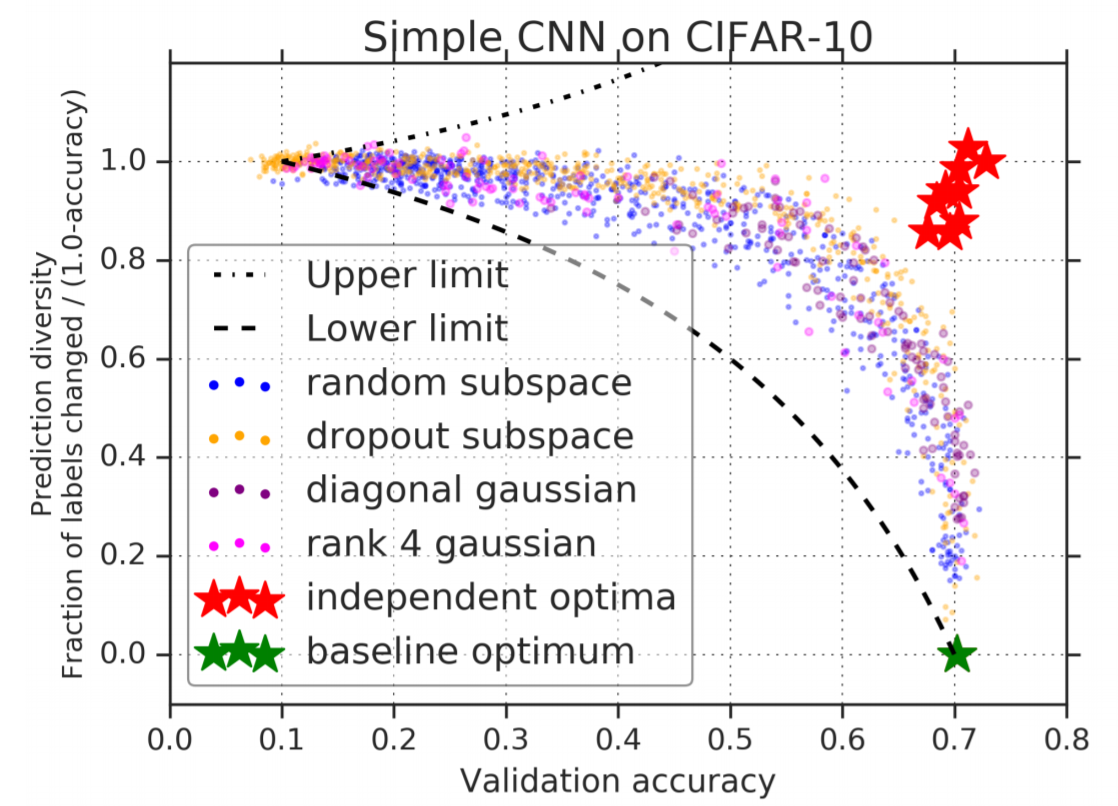
\includegraphics[width=0.7\linewidth]{./Figures/Figure6.png}
	\caption{Figure 6 left from the paper: 
		Y-axis is function disagreement of each sample with baseline optimum. Green star shows the single optimum: zero diversity because it is compared with itself. Dots show diversity (function disagreement) vs accuracy for the samples obtained via the 4 sampling techniques. For example, you can get more diverse predictions using the 4 sampling techniques by increasing the noise. But this comes at the cost of accuracy because you leave the loss valley shown in figure 5 of the paper and you visit a high-loss region. With red the predictions by different trajectories are shown. We can see that there is no trade off for different trajectories. We have similar accuracy and very different predictions.}
	\label{}
\end{figure}
\begin{figure}
	\centering
	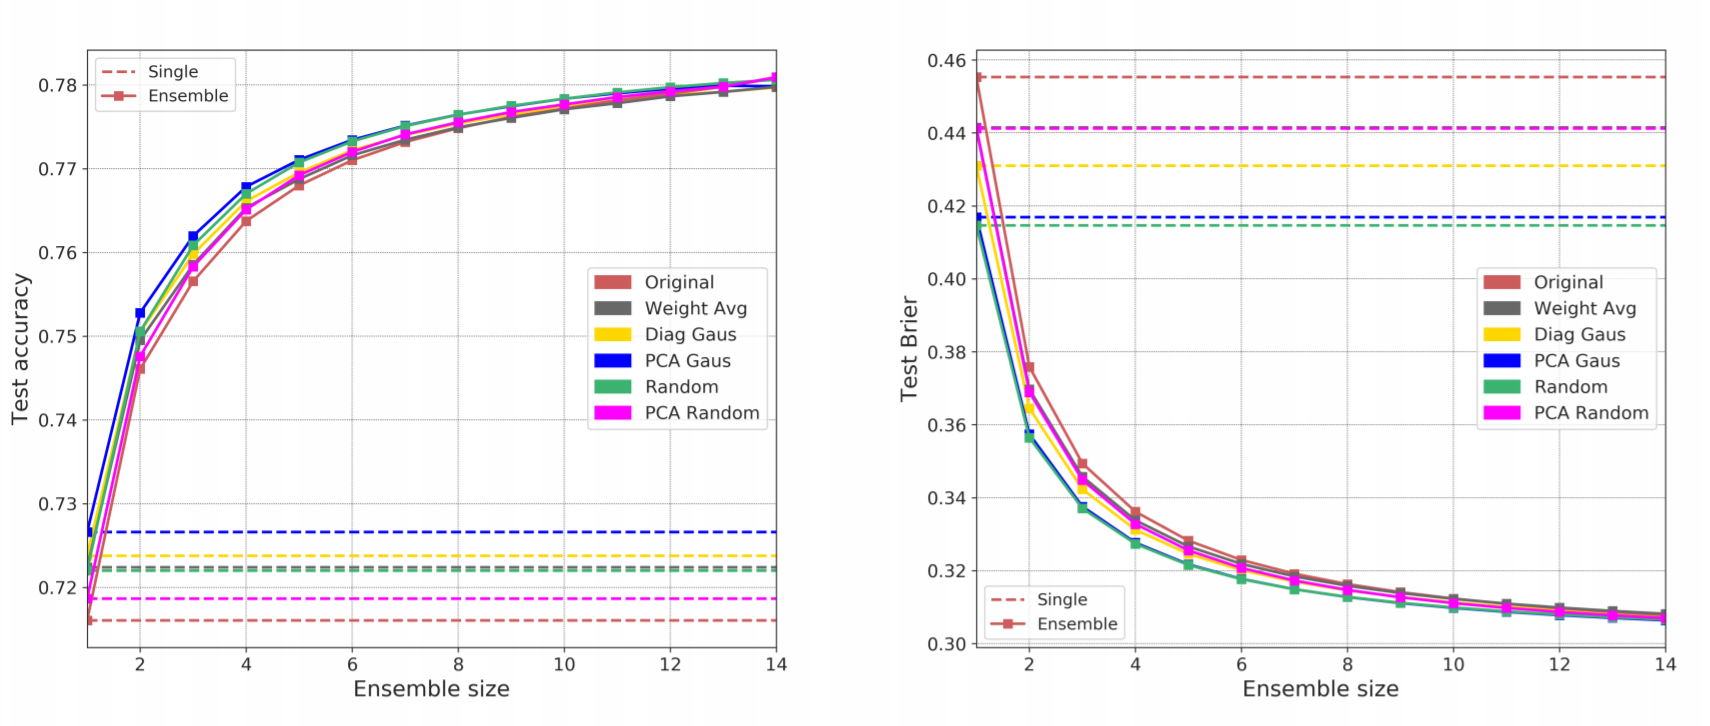
\includegraphics[width=1\linewidth]{./Figures/Figure8.png}
	\caption{Figure 8: 
		Left: Here the authors use deep ensembles plus additional samples via the 4 sampling techniques. Remember each optimum in the ensemble has an optimization trajectory that we can use to sample more weights using one of the 4 sampling techniques. What they do here is similar to Multi-SWAG proposed in \textcite{wilson2020bayesian}. It shows that ensembling plus sampling can be a little better than ensembling. Ensembling is for sure better than just sampling however in terms of generalization. Right: Same for calibration (uncertainty quality). Small Brier score means better calibrated uncertainty.}
	\label{}
\end{figure}

%%%%%%%%%%%%%%%%%%%%%%%%%%%%%%%%%%%%%%%%%%%%%%%%%%%%%%%%%%%%%%%%%%%%%%%%%%%%%%%%%%%%%%%%%%%%%%%%%%%%%%%%%	

%\section*{Appendix}
\newpage	
\printbibliography[heading=bibintoc,title={References}]
	
\end{document}